\documentclass[14pt]{extbook}
\usepackage{multicol, enumerate, enumitem, hyperref, color, soul, setspace, parskip, fancyhdr} %General Packages
\usepackage{amssymb, amsthm, amsmath, latexsym, units, mathtools} %Math Packages
\everymath{\displaystyle} %All math in Display Style
% Packages with additional options
\usepackage[headsep=0.5cm,headheight=12pt, left=1 in,right= 1 in,top= 1 in,bottom= 1 in]{geometry}
\usepackage[usenames,dvipsnames]{xcolor}
\usepackage{dashrule}  % Package to use the command below to create lines between items
\newcommand{\litem}[1]{\item#1\hspace*{-1cm}\rule{\textwidth}{0.4pt}}
\pagestyle{fancy}
\lhead{Progress Quiz 5}
\chead{}
\rhead{Version C}
\lfoot{8497-6012}
\cfoot{}
\rfoot{Summer C 2021}
\begin{document}

\begin{enumerate}
\litem{
For the scenario below, use the model for the volume of a cylinder as $V = \pi r^2 h$.
\begin{center}
    \textit{ Pringles wants to add 38 \text{percent} more chips to their cylinder cans and minimize the design change of their cans. They've decided that the best way to minimize the design change is to increase the radius and height by the same percentage. What should this increase be? }
\end{center}
\begin{enumerate}[label=\Alph*.]
\item \( \text{About } 11 \text{ percent} \)
\item \( \text{About } 3 \text{ percent} \)
\item \( \text{About } 19 \text{ percent} \)
\item \( \text{About } 17 \text{ percent} \)
\item \( \text{None of the above} \)

\end{enumerate} }
\litem{
Solve the modeling problem below, if possible.
\begin{center}
    \textit{ In CHM2045L, Brittany created a 23 liter 29 percent solution of chemical $\chi$ using two different solution percentages of chemical $\chi$. When she went to write her lab report, she realized she forgot to write the amount of each solution she used! If she remembers she used 15 percent and 37 percent solutions, what was the amount she used of the 15 percent solution? }
\end{center}
\begin{enumerate}[label=\Alph*.]
\item \( 14.64 liters \)
\item \( 10.14 liters \)
\item \( 11.50 liters \)
\item \( 8.36 liters \)
\item \( \text{There is not enough information to solve the problem.} \)

\end{enumerate} }
\litem{
Solve the modeling problem below, if possible.
\begin{center}
    \textit{ A new virus is spreading throughout the world. There were initially 4 many cases reported, but the number of confirmed cases has doubled every 1 days. How long will it be until there are at least 100000 confirmed cases? }
\end{center}
\begin{enumerate}[label=\Alph*.]
\item \( \text{About } 15 \text{ days} \)
\item \( \text{About } 5 \text{ days} \)
\item \( \text{About } 11 \text{ days} \)
\item \( \text{About } 6 \text{ days} \)
\item \( \text{There is not enough information to solve the problem.} \)

\end{enumerate} }
\litem{
Determine the appropriate model for the graph of points below.
\begin{center}
    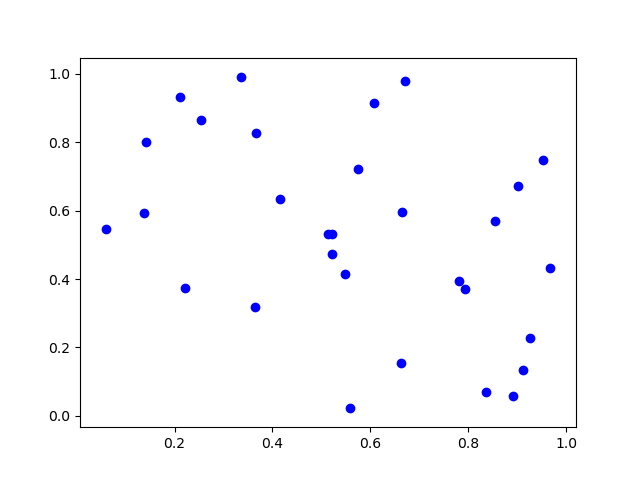
\includegraphics[width=0.5\textwidth]{../Figures/identifyModelGraph12C.png}
\end{center}
\begin{enumerate}[label=\Alph*.]
\item \( \text{Non-linear Power model} \)
\item \( \text{Linear model} \)
\item \( \text{Logarithmic model} \)
\item \( \text{Exponential model} \)
\item \( \text{None of the above} \)

\end{enumerate} }
\litem{
The temperature of an object, $T$, in a different surrounding temperature $T_s$ will behave according to the formula $T(t) = Ae^{kt} + T_s$, where $t$ is minutes, $A$ is a constant, and k is a constant. Use this formula and the situation below to construct a model that describes the uranium's temperature, $T$, based on the amount of time t (in minutes) that have passed. Choose the correct constant $k$ from the options below.
\begin{center}
    \textit{ Uranium is taken out of the reactor with a temperature of $180^{\circ}$ C and is placed into a $17^{\circ}$ C bath to cool. After 30 minutes, the uranium has cooled to $116^{\circ}$ C. }
\end{center}
\begin{enumerate}[label=\Alph*.]
\item \( k = -0.02473 \)
\item \( k = -0.01993 \)
\item \( k = -0.02514 \)
\item \( k = -0.01662 \)
\item \( \text{None of the above} \)

\end{enumerate} }
\litem{
For the scenario below, use the model for the volume of a cylinder as $V = \pi r^2 h$.
\begin{center}
    \textit{ Pringles wants to add 27 \text{percent} more chips to their cylinder cans and minimize the design change of their cans. They've decided that the best way to minimize the design change is to increase the radius and height by the same percentage. What should this increase be? }
\end{center}
\begin{enumerate}[label=\Alph*.]
\item \( \text{About } 13 \text{ percent} \)
\item \( \text{About } 8 \text{ percent} \)
\item \( \text{About } 9 \text{ percent} \)
\item \( \text{About } 14 \text{ percent} \)
\item \( \text{None of the above} \)

\end{enumerate} }
\litem{
Solve the modeling problem below, if possible.
\begin{center}
    \textit{ In CHM2045L, Brittany created a 15 liter 15 percent solution of chemical $\chi$ using two different solution percentages of chemical $\chi$. When she went to write her lab report, she realized she forgot to write the amount of each solution she used! If she remembers she used 7 percent and 37 percent solutions, what was the amount she used of the 37 percent solution? }
\end{center}
\begin{enumerate}[label=\Alph*.]
\item \( 7.50 liters \)
\item \( 11.00 liters \)
\item \( 5.62 liters \)
\item \( 4.00 liters \)
\item \( \text{There is not enough information to solve the problem.} \)

\end{enumerate} }
\litem{
Solve the modeling problem below, if possible.
\begin{center}
    \textit{ A new virus is spreading throughout the world. There were initially 5 many cases reported, but the number of confirmed cases has doubled every 2 days. How long will it be until there are at least 1000000 confirmed cases? }
\end{center}
\begin{enumerate}[label=\Alph*.]
\item \( \text{About } 36 \text{ days} \)
\item \( \text{About } 12 \text{ days} \)
\item \( \text{About } 11 \text{ days} \)
\item \( \text{About } 25 \text{ days} \)
\item \( \text{There is not enough information to solve the problem.} \)

\end{enumerate} }
\litem{
Determine the appropriate model for the graph of points below.
\begin{center}
    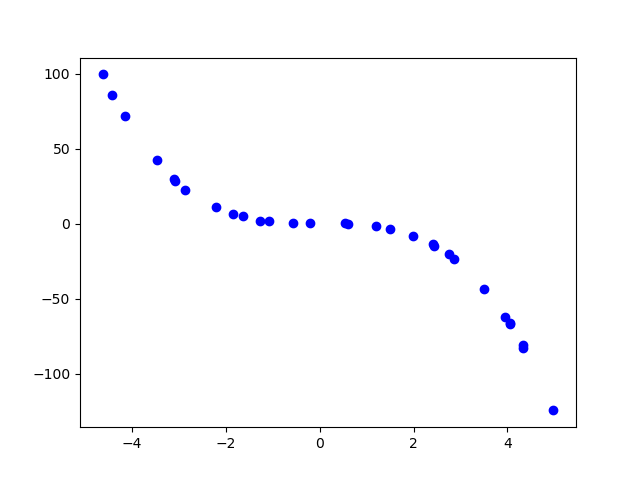
\includegraphics[width=0.5\textwidth]{../Figures/identifyModelGraph12CopyC.png}
\end{center}
\begin{enumerate}[label=\Alph*.]
\item \( \text{Exponential model} \)
\item \( \text{Non-linear Power model} \)
\item \( \text{Logarithmic model} \)
\item \( \text{Linear model} \)
\item \( \text{None of the above} \)

\end{enumerate} }
\litem{
For the scenario below, use the model for the volume of a cylinder as $V = \pi r^2 h$ to find the coefficient for the model of the new volume $V_{\text{new}} = k r^2 h$.
\begin{center}
    \textit{ Pepsi wants to increase the volume of soda in their cans. They've decided to decrease the radius by 15 percent and decrease the height by 14 percent. They want to model the new volume based on the radius and height of the original cans. }
\end{center}
\begin{enumerate}[label=\Alph*.]
\item \( k = 0.62135 \)
\item \( k = 0.00315 \)
\item \( k = 1.95203 \)
\item \( k = 0.00990 \)
\item \( \text{None of the above.} \)

\end{enumerate} }
\end{enumerate}

\end{document}